Example 1: 
To Make Parameteric candle Stand model in OpenSCAD using customizer

\begin{figure}[H] 
	\centering 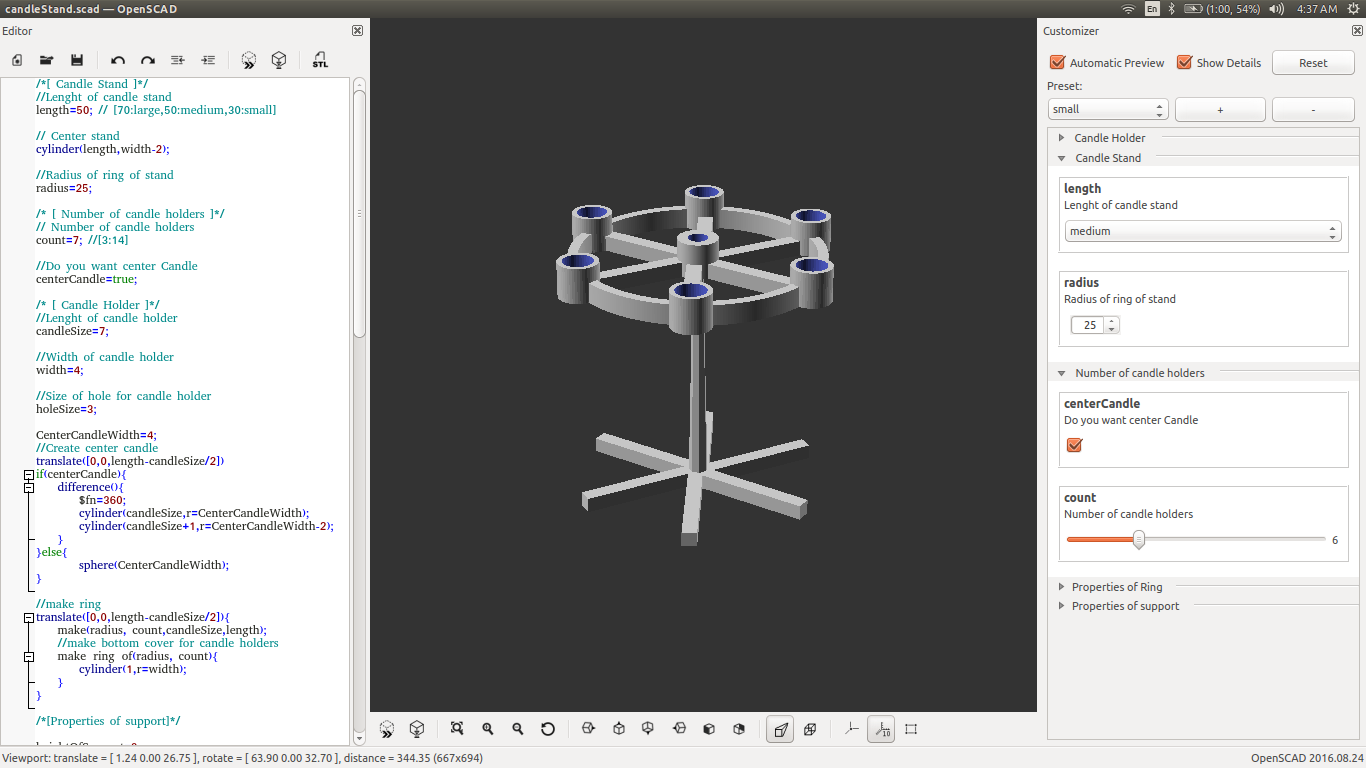
\includegraphics[scale=0.31]{images/output/9.png}
	\caption{Output of Code for Candle Stand model}
\end{figure}

\begin{lstlisting}[language=c++]
/*[ Candle Stand ]*/
//Lenght of candle stand
length=50; // [70:large,50:medium,30:small]

// Center stand
cylinder(length,width-2);

//Radius of ring of stand
radius=25;

/* [ Number of candle holders ]*/
// Number of candle holders
count=7; //[3:14]

//Do you want center Candle
centerCandle=true;

/* [ Candle Holder ]*/
//Lenght of candle holder
candleSize=7;

//Width of candle holder
width=4;

//Size of hole for candle holder
holeSize=3;

CenterCandleWidth=4;

/*[Properties of support]*/

heightOfSupport=3;
widthOfSupport=3;

/*[Properties of Ring]*/

heightOfRing=4;

widthOfRing=23;


//Create center candle
translate([0,0,length-candleSize/2])
if(centerCandle){
 difference(){
     $fn=360;
     cylinder(candleSize,r=CenterCandleWidth);
     cylinder(candleSize+1,r=CenterCandleWidth-2);
 }
}else{
     sphere(CenterCandleWidth);
}

//make ring 
translate([0,0,length-candleSize/2]){
 make(radius, count,candleSize,length);
 //make bottom cover for candle holders
 make_ring_of(radius, count){
     cylinder(1,r=width);
 }
}


//Base of candle stand
for (a = [0 : count - 1]) {
 rotate(a*360/count) {
 translate([0, -width/2, 0]) 
     cube([radius, widthOfSupport, heightOfSupport]);
 }
}

//make ring with candle holders
module make(radius, count,candleSize,length){
 
 $fa = 0.5;
 $fs = 0.5;
 difference(){
     union(){
          //making holders
         make_ring_of(radius, count){ 
             cylinder(candleSize,r=width);
         }
         
         //Attaching holders to stand
         for (a = [0 : count - 1]) {
             rotate(a*360/count) {
             translate([0, -width/2, 0]) 
                 cube([radius, widthOfSupport, heightOfSupport]);
             }
         }
         
         //make ring
         linear_extrude(heightOfRing)
         difference(){    
             circle(radius);
             circle(widthOfRing);
         }
     }
     //Making holes in candle holder
     make_ring_of(radius, count){
         cylinder(candleSize+1,r=holeSize);
     }
 }
}


module make_ring_of(radius, count){
 for (a = [0 : count - 1]) {
     angle = a * 360 / count;
     translate(radius * [cos(angle), -sin(angle), 0])
             children();
 }
}

// Written by Amarjeet Singh Kapoor <amarjeet.kapoor1@gmail.com>
//
// To the extent possible under law, the author(s) have dedicated all
// copyright and related and neighboring rights to this software to the
// public domain worldwide. This software is distributed without any
// warranty.
//
// You should have received a copy of the CC0 Public Domain
// Dedication along with this software.
// If not, see <http://creativecommons.org/publicdomain/zero/1.0/>.
\end{lstlisting}

